\chapter{Galaxy group algorithms}
\label{cha:galaxy_group_algorithms}
\minitoc%

As said previously, a good characterization of the galaxy environment implies a
good selection of galaxy groups. But galaxy observations are made in redshift
space, where the velocity dispersion of galaxies inside clusters stretch the
line-of-sight distribution of galaxies. Galaxies in a structure are not seen in
a local region of the space, but the structure is extended in larger range of
redshifts from the projected phase space, which is the only one accessible by
an observer.
\note{Add a citation to article.}
In consequence, the extraction of a galaxy group from the redshift space is
complex because a galaxy in the field can be associated to a group if it
pertains to the range of redshift of the group, and is inside the observational
cone formed by the virial radius. Such a galaxy is called an interloper (inside
the group by selection, but not pertaining to it in reality).
\note{Add the schema of the stage for it.}

A large number of group catalogues were constructed with a large panel of
method for selecting in order to go past the difficulties introduced by the
redshift distortions. A summary of some of such galaxy group algorithm follows,
with a description of their strengths and weaknesses.

\section{Some algorithms}
\label{sec:some_algorithms}

\subsection{\citet{Marinoni+02}}
\label{sub:marinoni02}

\subsubsection{Description}
\label{ssub:description}

This algorithm is a kind of modified version of the Friends-of-Friends
algorithm. The idea is to use over-densities of galaxies in the three
dimensional space (reconstructed simply from the redshift space), and use them
as potential centers for groups. Over-densities are estimated by use of a
Voronoi partition of space. The set of Voronoi cells forms a complete partition
of space, and the volume of a cell is inversely proportional to the galaxy
density around the galaxy in the cell. Then galaxies are sorted by decreasing
densities in order to use them as potential galaxy groups.

\begin{figure}
    \begin{minipage}{0.33\linewidth}
    \centering
    \subfloat[Convex hull]{%
        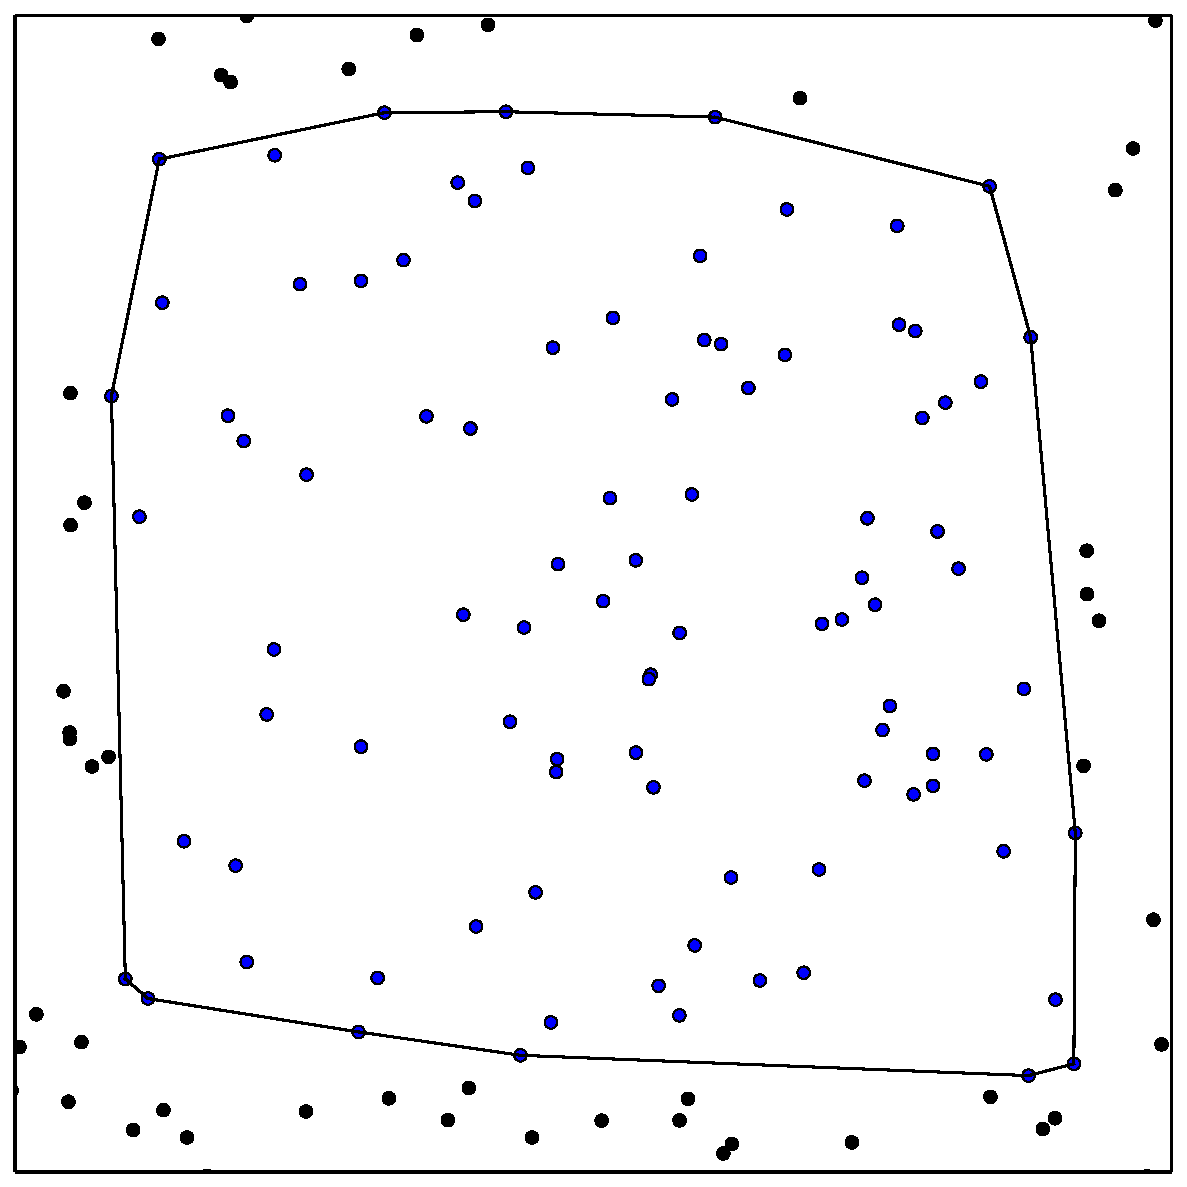
\includegraphics[width=\linewidth]{figures/algorithms/convex_hull.pdf}
    }
    \end{minipage}
    \begin{minipage}{0.33\linewidth}
    \centering
    \subfloat[Delaunay]{%
    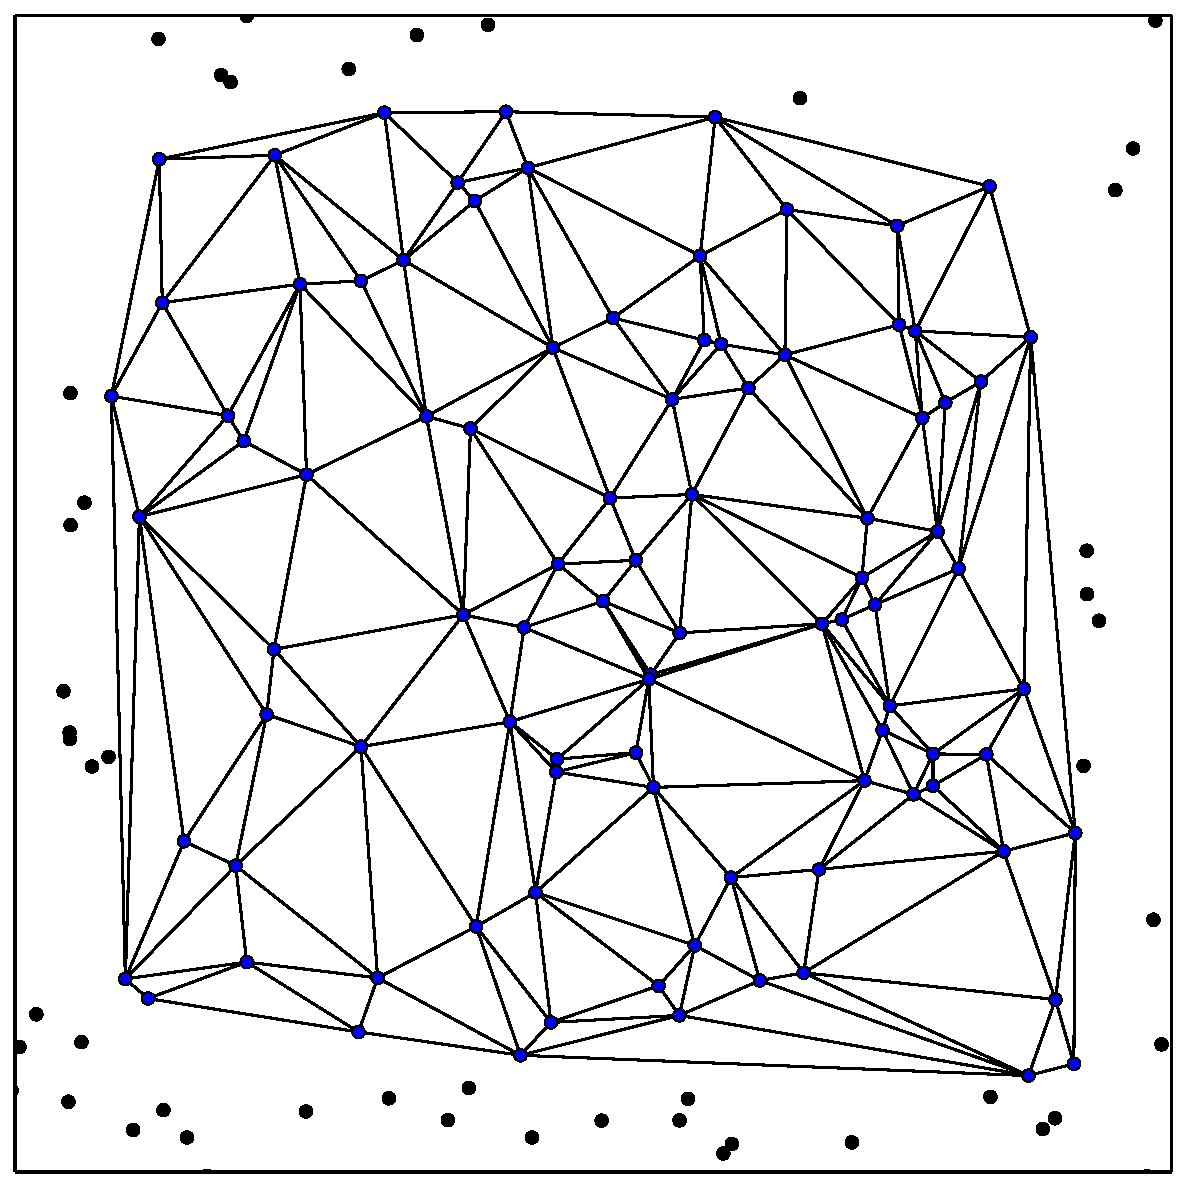
\includegraphics[width=\linewidth]{figures/algorithms/delaunay.pdf}
    }
    \end{minipage}
    \begin{minipage}{0.33\linewidth}
    \centering
    \subfloat[Voronoi]{%
    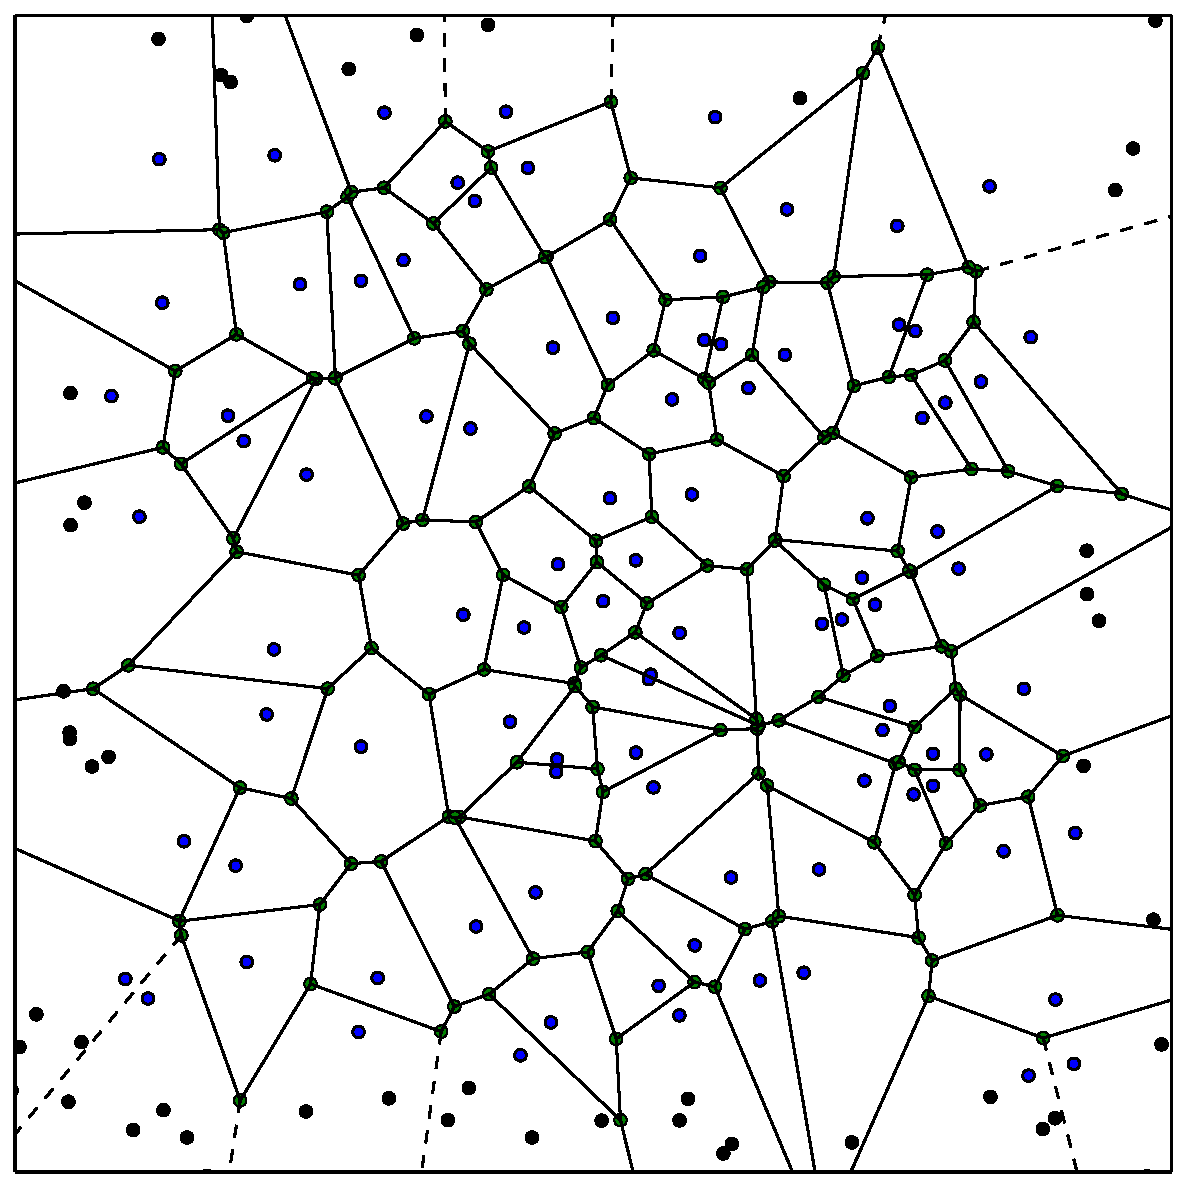
\includegraphics[width=\linewidth]{figures/algorithms/voronoi.pdf}
    }
    \end{minipage}
    \caption{Illustration of the tessellation of the space in a sub-sample of
        randomly positioned points. In \emph{black} the real point distribution
        (reflecting the real galaxy distribution) and in \emph{blue} the
        sub-sample used for the tessellation (reflecting the volume limited
        galaxy survey). (a) The convex hull is the set of points forming the
        hull of the sample. (b) The Delaunay mesh is represented by the lines
        interconnecting points. Each triangle of the mesh has his
        circumscribing circle without a point inside it by definition. (c) The
        Voronoi partition is the dual of the Delaunay mesh. Each node is the
        result of crossing median of the Delaunay mesh. Working on a sub-sample
        of galaxies shows that the Delaunay mesh is not well constrained at
    edges, and the Voronoi cells are affected too. A consequence is that their
volumes are biased and not corresponding to the real galaxy density around
them when too close to borders.\label{fig:convex_delaunay_voronoi}}
\end{figure}

The procedure for selecting galaxy groups is divided in three principal steps,
with an additional phase of initialization. The latter consists on the creation
of the Voronoi-Delaunay tessellation of the galaxy sample in three dimensional
space. For its construction, the idea is to generate a sample of coordinates in
a superior dimension by adding the distance to the origin of each points in it.
Then, the convex hull in this space is computed. It is the set of points
forming the hull of the sample. Projecting the convex hull to the initial space
returns the Delaunay mesh with the links between points. The Voronoi partition
is the dual of the Delaunay mesh and be can deduced from it. An illustration of
each set of points is given in \bartreffigure{convex_delaunay_voronoi}.

The first step is too search for potential groups by using the Voronoi
partition. Voronoi cells have the property that their volume is inversely
proportional to the density of points around each point. In case of galaxies,
this allows to access to local density around them. The detected high densities
in the three dimensional space are used as potential group centers. Galaxies
are sorted by increasing volume of their Voronoi cell, i.e.\ decreasing
density. \emph{First-order} galaxies, first linked to these potential groups,
are searched in a 1 Mpc region, using the Delaunay triangulation to access the
neighborhood of the group. If all first-order galaxies are already assigned to
another group, the two structures are merged.

The second step takes into account the redshift distortions, neglected in the
first step. For this, a cylindrical region is created with a base radius
perpendicular to the line-of-sight, and a height of around 20 Mpc. All galaxies
inside this region not already linked as first-order galaxies are second-order
galaxies. The size of the cylinder is chosen to take into account the redshift
elongation introduced in a typical group.

The third step uses the informations created from the two previous steps, which
are only a selection of potential groups. From the richness of those potential
groups, a relation between the richness and the cylinder lengths is deduced
since the the number of galaxies inside a group and its virial mass are
correlated. This implies that the group sample isn't affected by some
incompleteness, as the luminous one. From a constructed complete sub-sample,
the relation between the richness and the characteristics sizes of the cylinder
are deduced and modeled. Then, the second step is reapplied, the cylindrical
region inferred from the previous relations.

\subsubsection{Advantages and weaknesses}
\label{ssub:advantages}

The group extraction doesn't rely too much on physical assumptions as for the
FoF algorithm, but uses a geometrical approach, based directly on the galaxy
sample at disposition. Moreover, there is no free parameters, since the
cylindrical region is then adjusted, based on a relation between the virial
radius and the group richness. This relation is adjusted in a complete
sub-sample of galaxies to avoid incompleteness corrections, the algorithm
should be robust under different galaxy surveys.

But the Delaunay-Voronoi tessellation has some counterparts. The computation of
the Delaunay mesh is very difficult in non-Euclidean spaces, as the redshift
space, from the point of view of an observer. Moreover, the computation of the
volume of the Voronoi cell is complex too, especially with non-Euclidean
spaces. As a consequence, the computation must be done assuming that the
redshift space is perpendicular and fixed in space (in other words, the
line-of-sight direction at different location on the celestial sphere is the
same). Neglecting the celestial distortions limits the application of the
algorithm to a small portion of the sky of a few degrees of side.

In addition, border effects can't be neglected with the Voronoi partition of
space. Since Voronoi cells form a complete partition, cells at edges of the
galaxy sample have an infinite volume size. Also, the volume of cells close to
borders is biased because the distribution of galaxies is unknown beyond the
sample, and the Delaunay mesh can't be fully constrained to reflect the real
density of galaxies at edges. In other words, the volume of Voronoi cells near
edges doesn't really reflects the local density around galaxies, since the
galaxy distribution is unknown beyond the limit of the sample.

Finally, the tessellation is computed for a flux-limited sample of galaxies,
but the density around galaxies is used to search high mass halos first. Since
the luminous incompleteness is decreasing the observed number of galaxies with
increasing redshift, the effect is that nearby groups are searched first. With
the redshift distortions, the consequences of such bias in the selection aren't
trivial to understand on the resulting group catalogue.

In conclusion, the Voronoi-Delaunay method of \citet{Marinoni+02} can't be
really applied to recent galaxy surveys covering a large area of the sky.

\subsection{\citet{Yang+07}}
\label{sub:yang07}

This algorithm takes into account our knowledge on the large scale structure
extracted from the cosmological simulations to improve the grouping of
galaxies. In particular, an assumption is made on the galaxy density profile
inside halos to follow \citet{NFW+97} to define a parameter used to assign
galaxies to groups. A density contrast parameter is defined as the ratio
between the projected density of galaxies inside an halo and the density of
field galaxies (which are the interlopers). Higher is this ratio, higher the
galaxy is likely to belong to the group. The density of galaxies in the halo is
simply the integration of the distribution function along the line-of-sight,
and for interlopers, its the integration of the mean density of the Universe
along the line-of-sight over the Hubble distance. This results in th following
definition for the density contrast:
%
\begin{equation}
    P_M \left(R, \Delta z\right)=\cfrac{H_0}{c} \cfrac{\Sigma
    \left(R\right)}{\overline{\rho}} p \left(\Delta z\right)
\end{equation}
%
where $H_0$ is the Hubble constant, $c$ the speed of light,
$\Sigma\left(R\right)$ the projected surface density of galaxies at the
projected radius $R$, $\overline{\rho}$ the mean density of the Universe and $p
\left(\Delta z\right)$ is the velocity distribution of galaxies in terms of
redshift differences $\Delta z$ with the group redshift. This definition is
problematic: the density of interlopers is assumed to be constant and the same
for all halos. But as described in \citet{MBM+10}, the density of interlopers
is related to the position in the halo, and their velocity distribution isn't
flat.

Using this density contrast criterion implies to have potential groups on which
to apply it. For this, initially, a FoF algorithm is done on the galaxy sample
but with very small linking lengths. This potential groups are seed whose
membership must be updated using the density contrast, as described below.

For each group, its virial mass is estimated from a relation between the group
luminosity and its mass. Initially, this is a constant ratio, then adjusted on
the group sample itself. From it, the density contrast can be computed for each
galaxy on each group. A galaxy is assigned to a group if $P_M>B$ were $B$ is a
threshold. If this condition is satisfied for multiple groups, it is assigned
to the group with the highest $P_M$.

Then group centers and luminosities are recomputed with the new membership,
iterating over the previous step until a convergence in the membership is
observed.

Once the convergence is reached, the relation between the virial mass and the
luminosities of groups is recomputed by abundance matching between the
distribution of group luminosities obtained from the sample and the expected
distribution of virial masses assuming an halo mass function. Then the previous
iterative process is done again, and this goes until a convergence is reached
for the relation.

The algorithm have some lacks that should be technically and physically
corrected to be good enough in the group extraction. Indeed, some incoherences
are present in the implementation of the grouping algorithm. For example, the
given formula for the computation of the virial radius is done for halos being
over-densities of $\Delta=180$ of the mean density of the Universe, while the
computation of the abundance matching is done with the halo mass function of
\citet{Warren+06} for the FoF mass of halos from the cosmological simulation
used. The difference between the FoF mass and the virial mass is significant
and should be taken into account in the grouping process.

\subsection{\citet{DominguezRomero+12}}
\label{sub:dominguezromero12}

This algorithm is an adaptation of \citet{Yang+07}, based on a better Bayesian
approach, noting that the grouping method of \citet{Yang+07} is simply a
learning algorithm called K-means. Instead of assigning in an hard way galaxies
to groups in the iterative process, this method assigns responsibilities,
equivalents of a probability of belonging to a group, pondered over all groups
in the sample, using the density contrast definition above as some probability
to be in the group.

First, potential groups are estimated assuming that the most luminous galaxies
are linked to most massive systems. Then, galaxies are assigned to a group as
satellites members if they have a density contrast superior to a chosen low
threshold to allow a maximum of galaxies to belong to the group, without
introducing too much interlopers since their responsibilities will be low and
won't affect group properties. As for \citet{Yang+07}, an iteration over the
membership and the relation used to compute virial properties is done until
convergence. Finally, galaxies are hardly assigned to a group, the one for
which the responsibility is the highest.

Inconvenient of this method are essentially inherited from \citet{Yang+07}.

\subsection{\citet{MunozCuartas+12}}
\label{sub:munozcuartas12}

This method is similar to the FoF algorithm, but applied directly on halos and
not on galaxies. From an initial set of halos, a maximal circular radius is
computed from the virial radius in the transverse direction to the
line-of-sight. A maximal length of search for the redshift dimension is
estimated from the circular velocity of the halo. Those halos are sorted by
decreasing masses. For each one, other halos (and their galaxies) are merged
into the current halo if they belong to the ellipsoid defined by the two
lengths defined above, centered on the halo.

Then, group properties are computed from the membership obtained previously.
The new virial masses are evaluated with an abundance matching between the
group stellar masses and the halo mass function. The iteration is stopped once
the number of halos doesn't change.

This method doesn't have any free parameter and doesn't rely on too much
assumptions and models. Only the abundance matching can be responsible for a
bias, since the virial mass is crucial in the merging of halos. As mentioned by
\citet{Yang+07}, the one-to-one assumption of the abundance matching creates an
intrinsic dispersion in the mass estimation that is relatively low, and thus
should not affect the galaxy grouping.

\section{Discussion}
\label{sec:gga_discussion}

We can extract common principles of the different algorithms we described
above. There are two approaches for the galaxy grouping: a geometrical one
based only on the positional informations of galaxies and a Bayesian one using
priors on group properties and galaxies therein. What emerged is that a large
majority of these algorithms make a harmonious combination of these approaches
in order to conserve only their strengths. A typical geometrical algorithm is
the Friends-of-Friends (see \bartrefchapter{friends_of_friends_algorithm}),
linking galaxies between them if they are closer than a linking length. This
method has the default of creating bridges between two different galaxy groups
if two of their members are closer than the linking length. Adding priors to
such a scheme, the membership can be improved by breaking the problematic
bridges. This is a good summary for the method of \citet{Marinoni+02} or
\citet{MunozCuartas+12}. Moreover, the bias in distance introduced by redshift
can be reduced with same prescriptions ad done in \citet{Liu+08}.

\begin{figure}[htb]
    \centering
    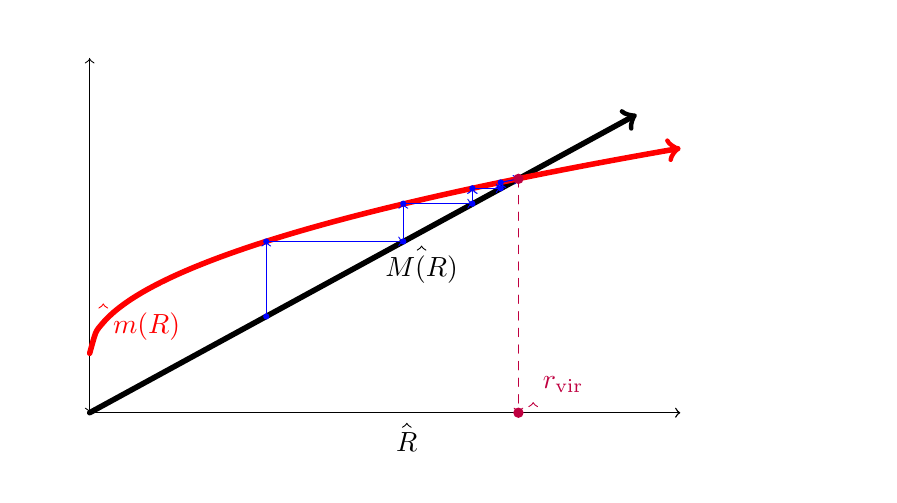
\begin{tikzpicture}[line cap=round,line join=round,->=triangle 45,x=1.0cm,y=1.0cm,scale=0.75]
        \clip(-1.05,-1.06) rectangle (13.19,6.52);
        \draw (0,6)-- (0,0);
        \draw (0,0)-- (10,0);
        \draw [line width=2pt,color=black] (0,0)-- (9.26,5.05);
        \draw [->] (0,0) -- (10,0);
        \draw [->] (0,0) -- (0,6);
        \draw[line width=2pt,color=red, smooth,samples=100,domain=0.00001:10.0] plot (\x, {1.1*\x^(0.5)+1}) ;
        \draw [->,color=blue] (2.99,1.63) -- (2.99,2.9);
        \draw [->,color=blue] (2.99,2.9) -- (5.31,2.9);
        \draw [->,color=blue] (5.31,2.9) -- (5.31,3.54);
        \draw [->,color=blue] (5.31,3.54) -- (6.48,3.54);
        \draw [line width=0.5pt,color=blue] (6.48,3.54) -- (6.48,3.8);
        \draw [->,color=blue] (6.48,3.8) -- (6.96,3.8);
        \draw [line width=0.5pt,color=blue] (6.96,3.8) -- (6.96,3.9);
        \draw [->,color=blue] (6.96,3.9) -- (7.26,3.96);
        \draw [dash pattern=on 3pt off 3pt,color=purple] (7.26,3.96)-- (7.26,0);
        \draw[color=black] (5.62,2.83) node[below] {$M(R)$};
        \draw[color=black] (5.37,-0.17) node[below] {$R$};
        \draw[color=red] (0.23,1.85) node[below right] {$m(R)$};
        \fill [color=blue] (2.99,1.63) circle (1.5pt);
        \fill [color=blue] (2.99,2.9) circle (1.5pt);
        \fill [color=blue] (5.31,2.9) circle (1.5pt);
        \fill [color=blue] (5.31,3.54) circle (1.5pt);
        \fill [color=blue] (6.48,3.54) circle (1.5pt);
        \fill [color=blue] (6.48,3.8) circle (1.5pt);
        \fill [color=blue] (6.96,3.8) circle (1.5pt);
        \fill [color=blue] (6.96,3.9) circle (1.5pt);
        \fill [color=purple] (7.26,3.96) circle (2.5pt);
        \fill [color=purple] (7.26,0) circle (2.5pt);
        \draw[color=purple] (7.51,0.18) node[above right] {$r_{\mathrm{vir}}$};
    \end{tikzpicture}
    \caption{Graph illustrating the convergence of the group membership by
    iterations.\label{fig:convergence}}
\end{figure}

Iteration seems to be a key in a good grouping algorithm. A convergence in the
galaxy membership is assured by updating group properties along iterations, and
using it to constrain the selection. The convergence in various scaling
relations in groups is also assured by iterations, giving a self-consistency of
the clustering with the data itself: galaxy group algorithms are special kind
of machine learning algorithm. For example, we suppose an algorithm using a
relation between the stellar mass of groups and its virial mass (see
\bartreffigure{convergence}). The stellar mass of the group in red increases
with the projected radius since the number of galaxies inside it increases.
There is also a relation between projected radius and virial mass. Starting
with an initial guess for the virial mass, we can perform a galaxy selection
and estimate a stellar mass for the group. With the relation, we can make a new
estimation of the virial mass. This process goes until the convergence
represented by the virial radius $r_\mathrm{vir}$ in
\bartreffigure{convergence}.

The Bayesian approach used in the described galaxy group algorithms as also its
counterparts: if the chosen models are bad, the clustering will be affected
too. For example, \citet{Yang+05} assumes a flat line-of-sight velocity
dispersion and a flat distribution of interlopers in the computation of density
contrast, which clearly depends on the projected radius pointed by the
observer. Another problem is the way to test such algorithms. Previously
described algorithms were tested on different galaxy mock catalogues, not
constructed in the same way, without the same physics applied inside them. In
consequence the comparison is very difficult because not operated in the same
conditions. And the definition of an optimal extraction, and the statistics
used assess their perfomances differ with galaxy group algorithm developers.

To go beyond such limitations that will never be completely avoided,
a probabilistic approach of galaxy groups seems to be a good compromised (see
\bartrefchapter{MAGGIE}). Moreover, the tests for algorithms must be well
defined, with a common galaxy mock catalogue to perform the comparisons and a
good definition of the statistics to use. How well are recovered galaxy groups?
How well they are polluted by interlopers? How many selected groups are
spurious? How virial properties of the parent halo are recovered? How scaling
relations are recovered? They are the questions to answer in order to
characterize the quality of a grouping algorithm.

% vim: set tw=79 :
